\chapter{CrazyMARL}
We present \textbf{CrazyMARL}, an end-to-end JAX-based pipeline for training multi-agent reinforcement learning (MARL) policies on teams of Crazyflie quadrotors. Our framework seamlessly handles both single-vehicle and cooperative multi-agent tasks, including scenarios with cable-suspended payloads. At its core, the simulation leverages the high‐performance MJX backend of the MuJoCo physics engine, interfaced through the Brax library for highly parallelized training. Our environments and algorithms are based on JaxMARL introduced by \autocite{flair2023jaxmarl}. We expose the simulator as a \texttt{JAXMARL.Mabrax} environment, providing a drop-in API for JAX-based RL algorithms.

\section{Simulation Environment}
The simulation environment is built upon MuJoCo's XML specification and the GPU-accelerated MJX solver. We adopt a modular, extensible design in which each scenario is defined by auto-generated XML descriptors. These files specify vehicle geometries, inertial properties, cable parameters, payload characteristics, and any static or dynamic obstacles. A lightweight Python utility reads a user‐defined configuration (YAML or JSON) and generates the corresponding XML, allowing researchers to rapidly prototype new dynamics or collaborative tasks. \todo{more details on configuration and generation of the XML files.}
\subsection{Environment Reset}
\begin{figure}
    \centering
    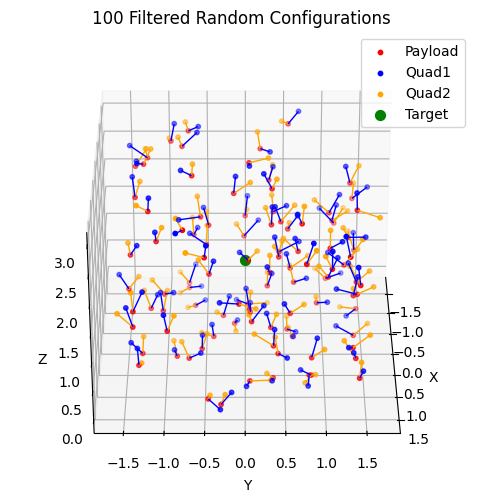
\includegraphics[width=0.5\textwidth]{reset_config.png}
    \caption{Example of the random reset configuration.}
    \label{fig:reset_config}
\end{figure}
At each reset, the payload center~$p$ is sampled uniformly in
\[
p_{xy}\sim\mathcal{U}([-L,L]^2),\quad p_z\sim\mathcal{U}([-Z,Z]),
\]
Then we use the payload position $p$ as the center point and randomly sample $N$ quadrotors in a spherical shell around the payload. The radius $r_i$ of each quadrotor is sampled from a normal distribution with mean $\mu_r$ and standard deviation $\sigma_r$, and then clipped to cable length. The angles $\theta_i$ and $\phi_i$ are sampled from normal distributions with means $\mu_\theta$ and $\phi_{\mathrm{offset}}$ respectively, and standard deviations $\sigma_\theta$ and $\sigma_\phi$. The angles are then adjusted to ensure they are within the range $[0, 2\pi]$. The equations for sampling the quadrotor positions are as follows:
\[
r_i = \mathrm{clip}\bigl(\mu_r+\sigma_r\varepsilon_i^{(r)},\,r_{\min},\,r_{\max}\bigr),\quad
\theta_i = \mu_\theta+\sigma_\theta\varepsilon_i^{(\theta)},\quad
\phi_i = \tfrac{2\pi(i-1)}{N} + \phi_{\mathrm{offset}} + \sigma_\phi\varepsilon_i^{(\phi)},
\]
where $\varepsilon_i^{(\cdot)}\!\sim\mathcal{N}(0,1)$, $\phi_{\mathrm{offset}}\!\sim\mathcal{U}(-\pi,\pi)$, and
\[
\mu_r=c,\;\sigma_r=\tfrac{c}{3},\;r_{\min}=0.05,\;r_{\max}=c,\;
\mu_\theta=\tfrac{\pi}{7},\;\sigma_\theta=\tfrac{\pi}{8},\;\sigma_\phi=\tfrac{\pi}{N+1}.
\]

These are converted to Cartesian positions
\[
q_i = p + r_i
\begin{bmatrix}
\sin\theta_i\cos\phi_i\\
\sin\theta_i\sin\phi_i\\
\cos\theta_i
\end{bmatrix},
\]
\todo{fix equations}
with the $z$–coordinate clipped. 
This results in a even distribution of valid initial configurations, also including starting from the ground as shown in \autoref{fig:reset_config}. 





\subsection{Quadrotor}
% - Modeling of quadrotor with thrust based on work of https://github.com/google-deepmind/mujoco_menagerie/blob/main/bitcraze_crazyflie_2/cf2.xml
- Describe thrust on quadrotor
- Motor Model

\subsection{Cable Suspended Payload}
- Description of cable suspended payload modeling with tendons or cables
% \subsection{Obstacles}
\subsection{Simulation Parameters}
- Configuration of simulation with initial position wind etc

\section{Observation Space}
- Description of the observation space for single quadrotor
- Description of the team reward components
% \subsection{Payload Representations}
% \subsection{Obstacle Representations}
\subsection{Observation Space Design}
- Ideas used for observation space
\subsection{Multi-Agent Observation Mapping}
- How is the full state mapped to single agents in the JAXMARL env

\section{Action Space}
- Actions always the 4 thrusts mapped from -1 to 1

\section{Domain Randomization}
\subsection{Environment Reset}

\subsection{Hardeware Rollout}

